% !TeX spellcheck = en_US

\chapter{Results}
\label{chap:results}
For this project we've chosen \CC17 as the programming language to implement an efficient, multi-threaded program to achieve a better performance. The whole training process has been run on a cluster of $9$ identical machines with \texttt{Intel(R) Xeon(R) CPU E5430 @ 2.66GHz - 16GB RAM}. With this computational power, we have been able to perform multiple experiments with a variable parameter $K$ in the $K$-fold external cross-validation: $2$, $3$, $5$, $10$, $20$, $50$, $150$, $300$, $750$. The whole computation took a period of seven days. We have been able to calculate the various losses for each single epoch (aka parameter $T$ of AdaBoost and Bagging).\\
The program has been written to dump all the results in a \texttt{json} file, in order to then extract useful information though some scripts written in Python. In all of the experiments, both AdaBoost and Bagging have been trained over the whole data-set.\\
\begin{figure}
	\centering
	\subfloat[K = 2]{
		\label{ref_k2}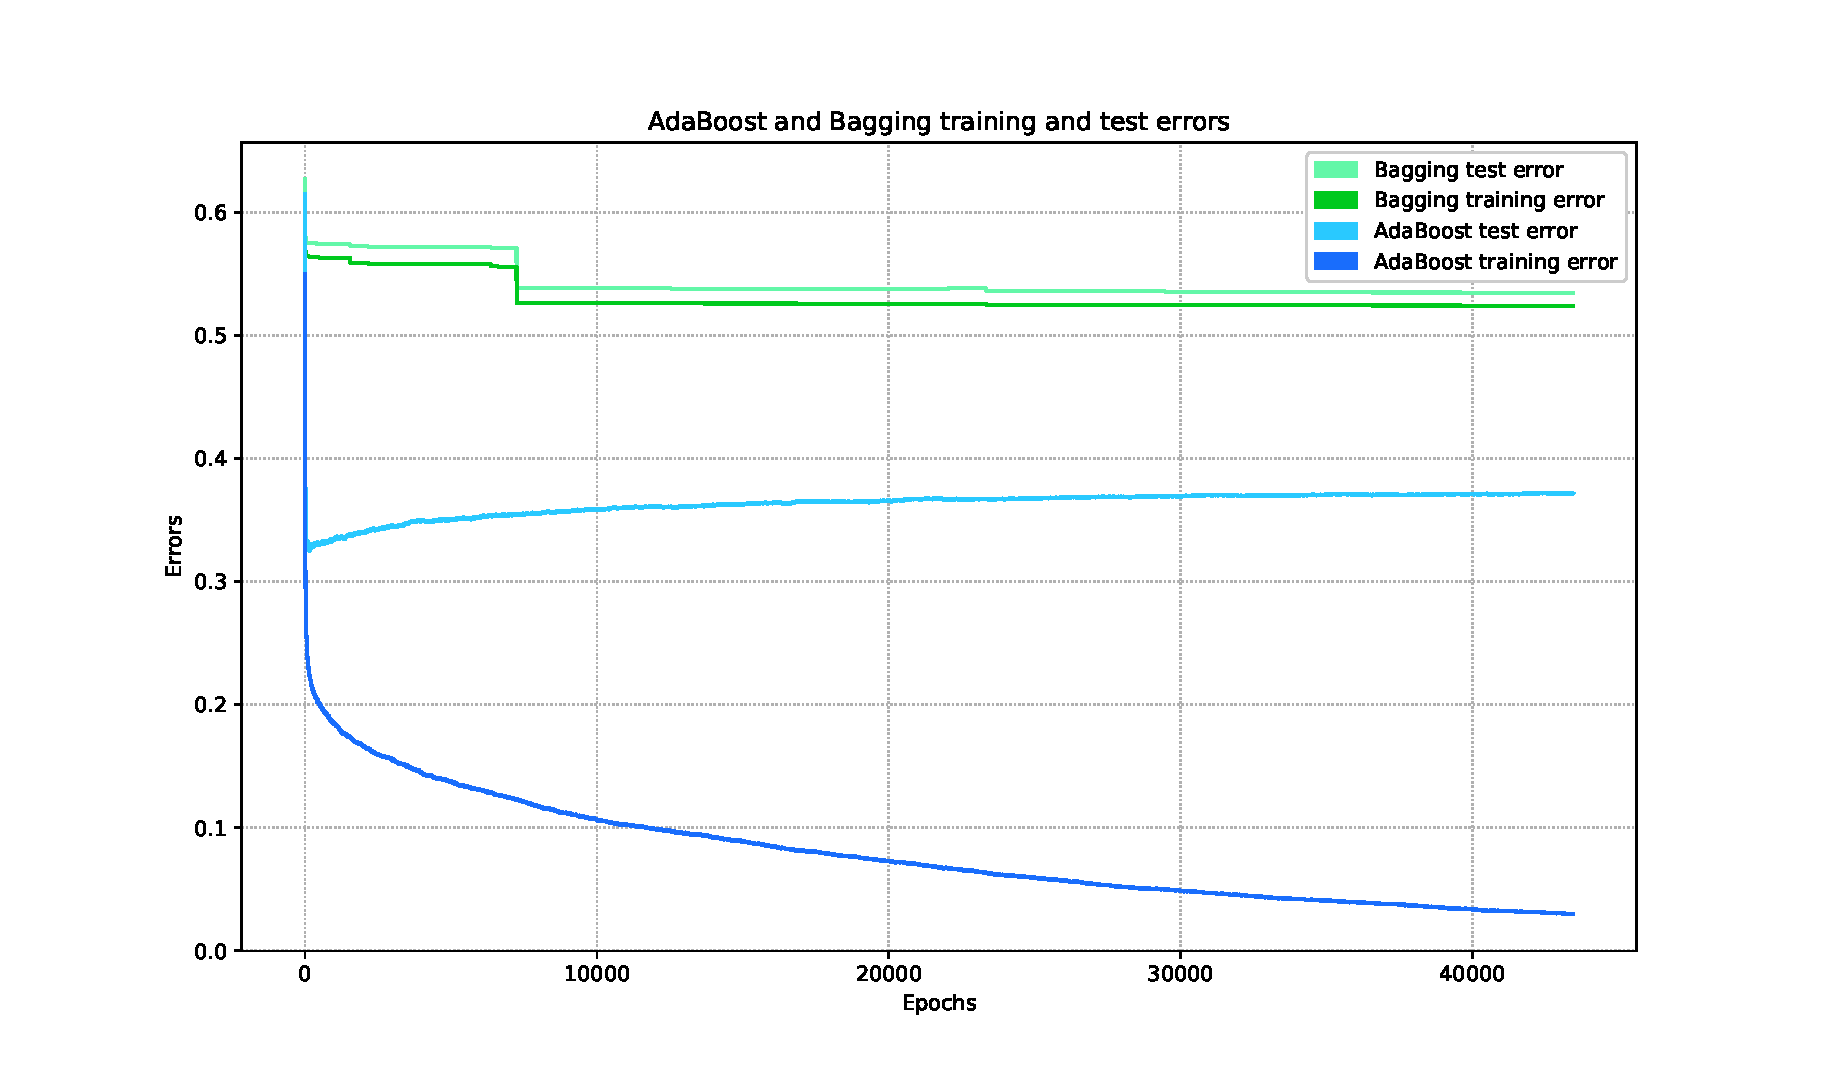
\includegraphics[width=0.5\textwidth]{figs/report_k2.eps}
	}
	\subfloat[K = 5]{
		\label{ref_k5}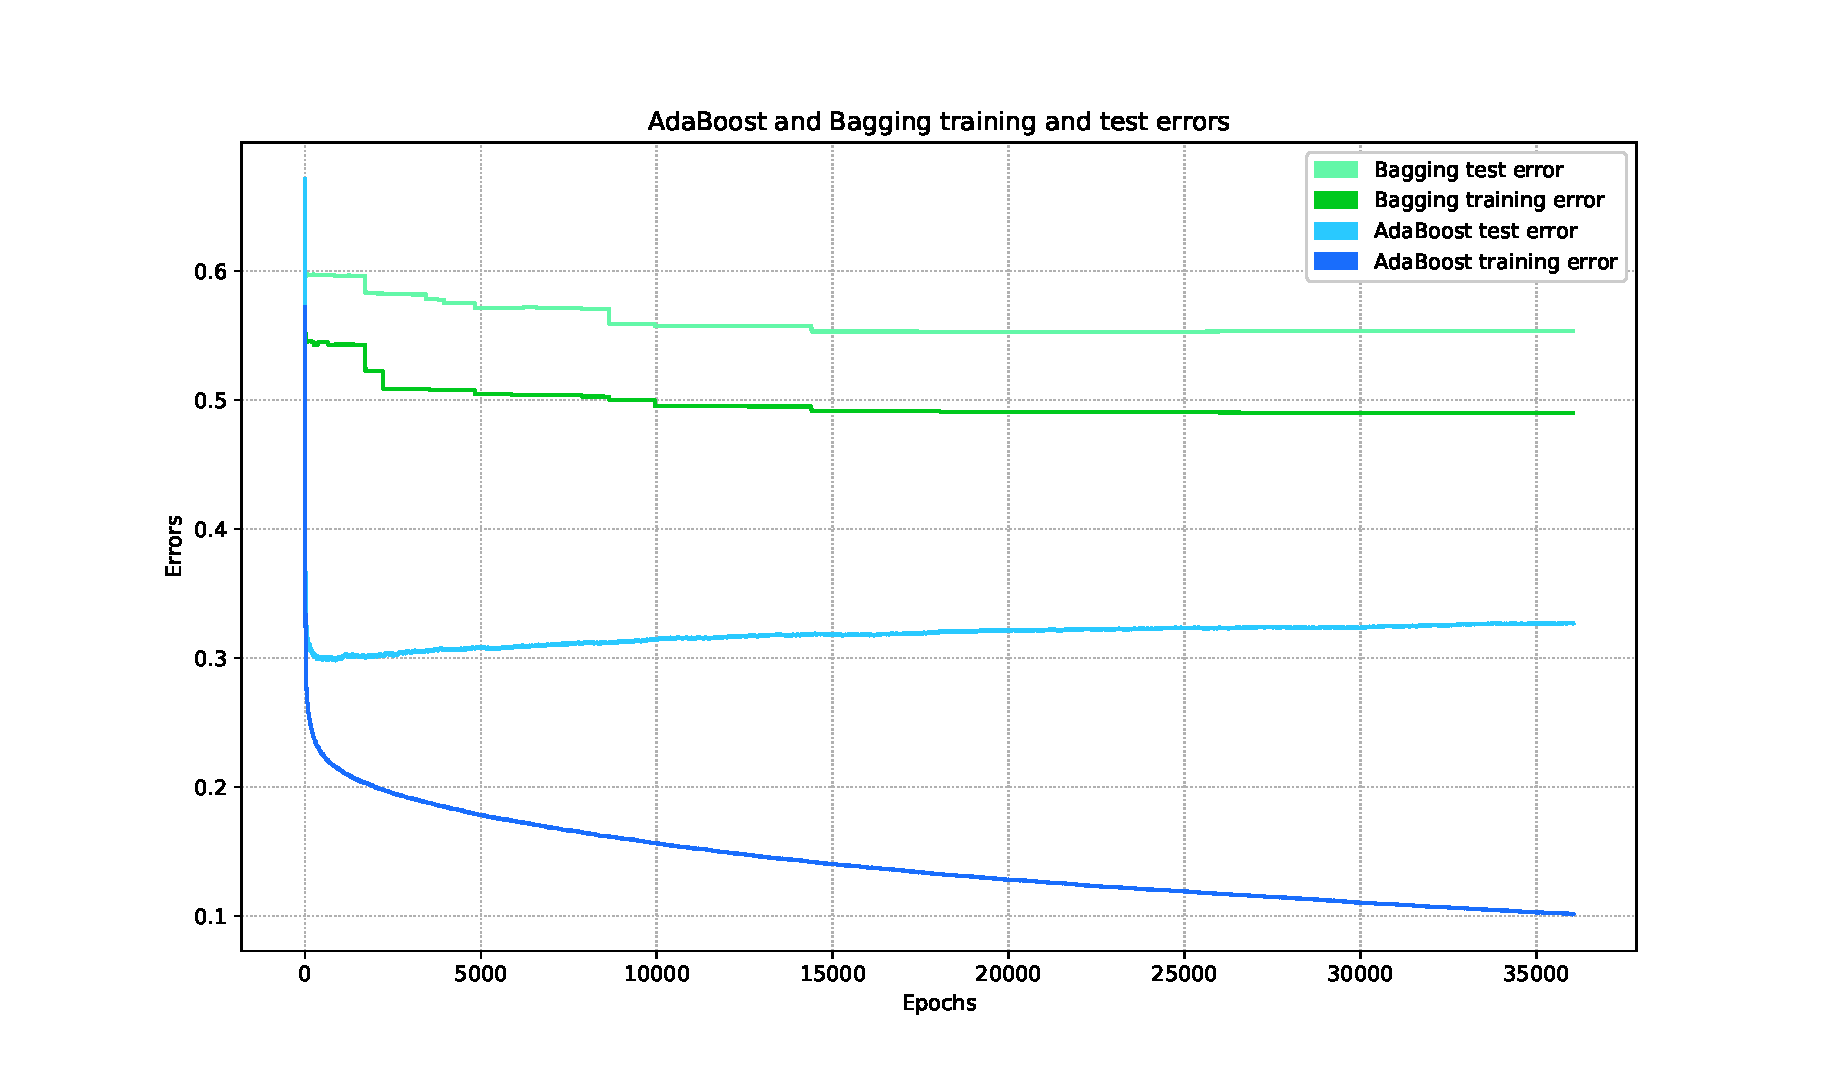
\includegraphics[width=0.5\textwidth]{figs/report_k5.eps}
	}
	\\
	\subfloat[K = 20]{
		\label{ref_k20}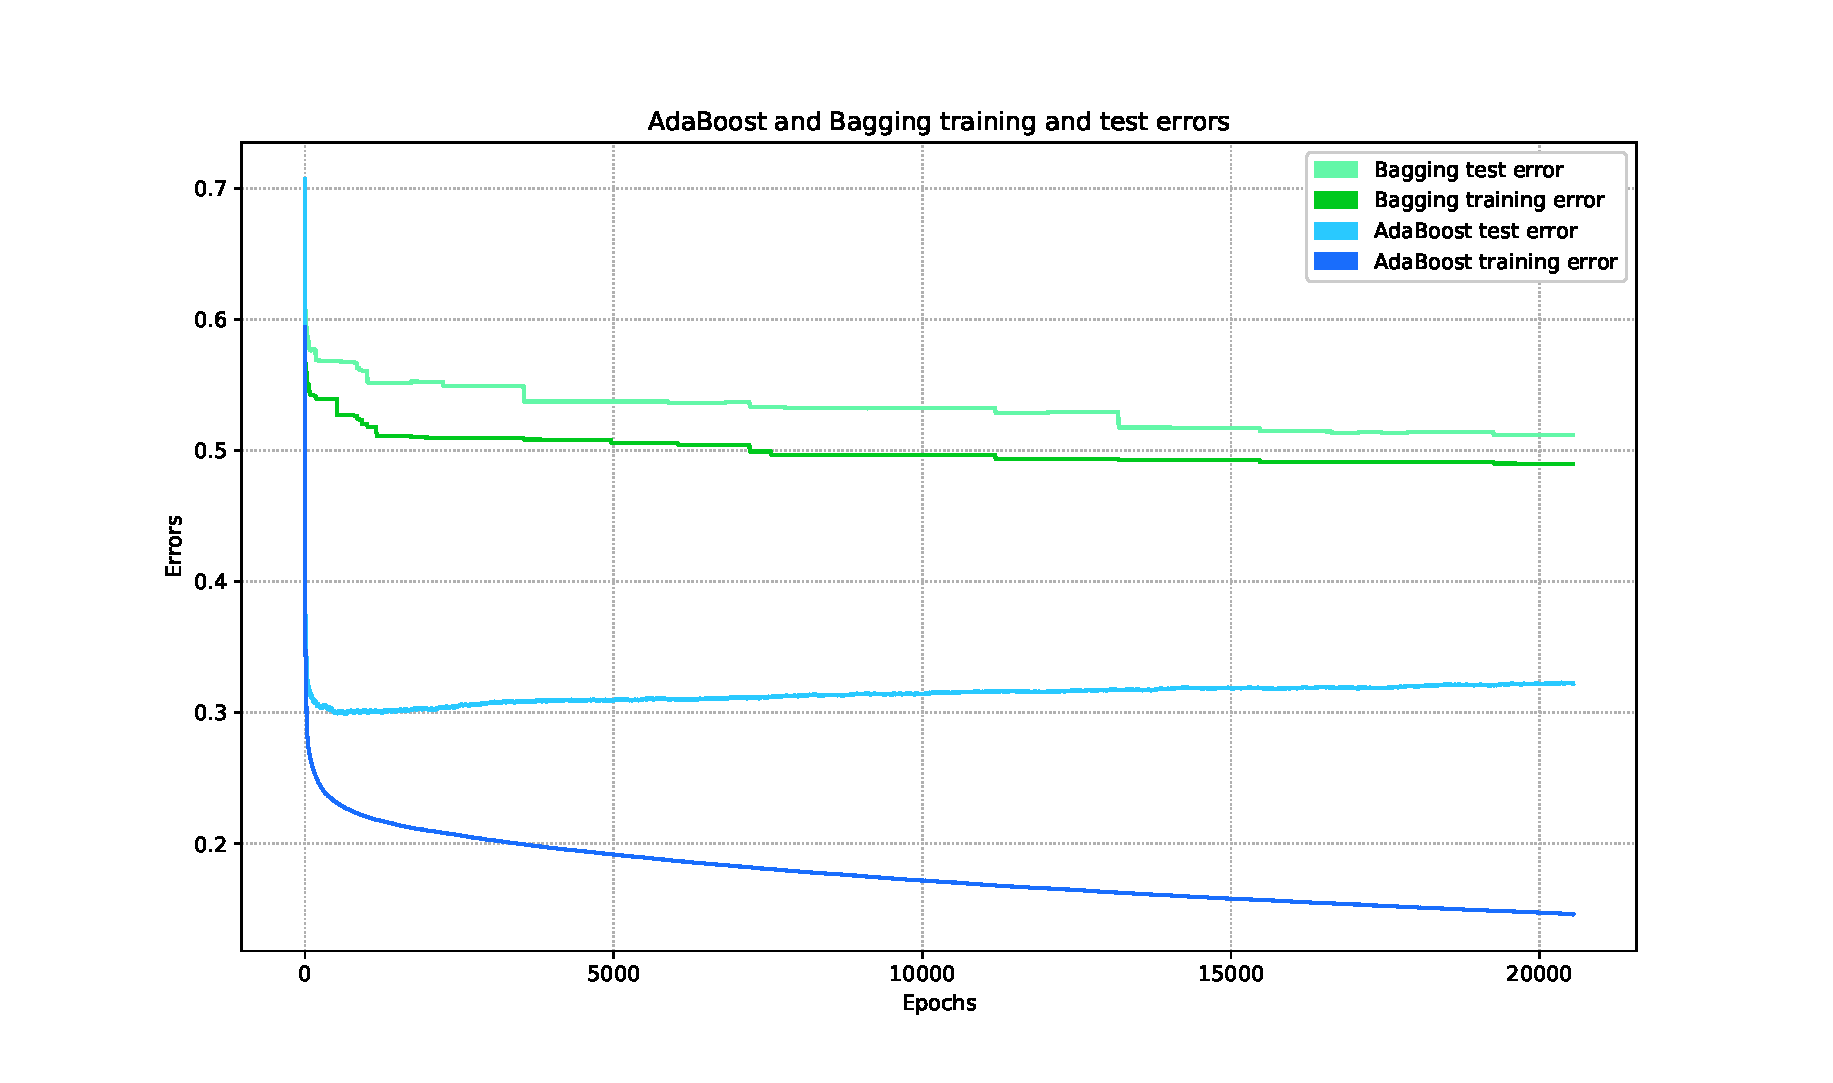
\includegraphics[width=0.5\textwidth]{figs/report_k20.eps}
	}
	\subfloat[K = 750]{
		\label{ref_k750}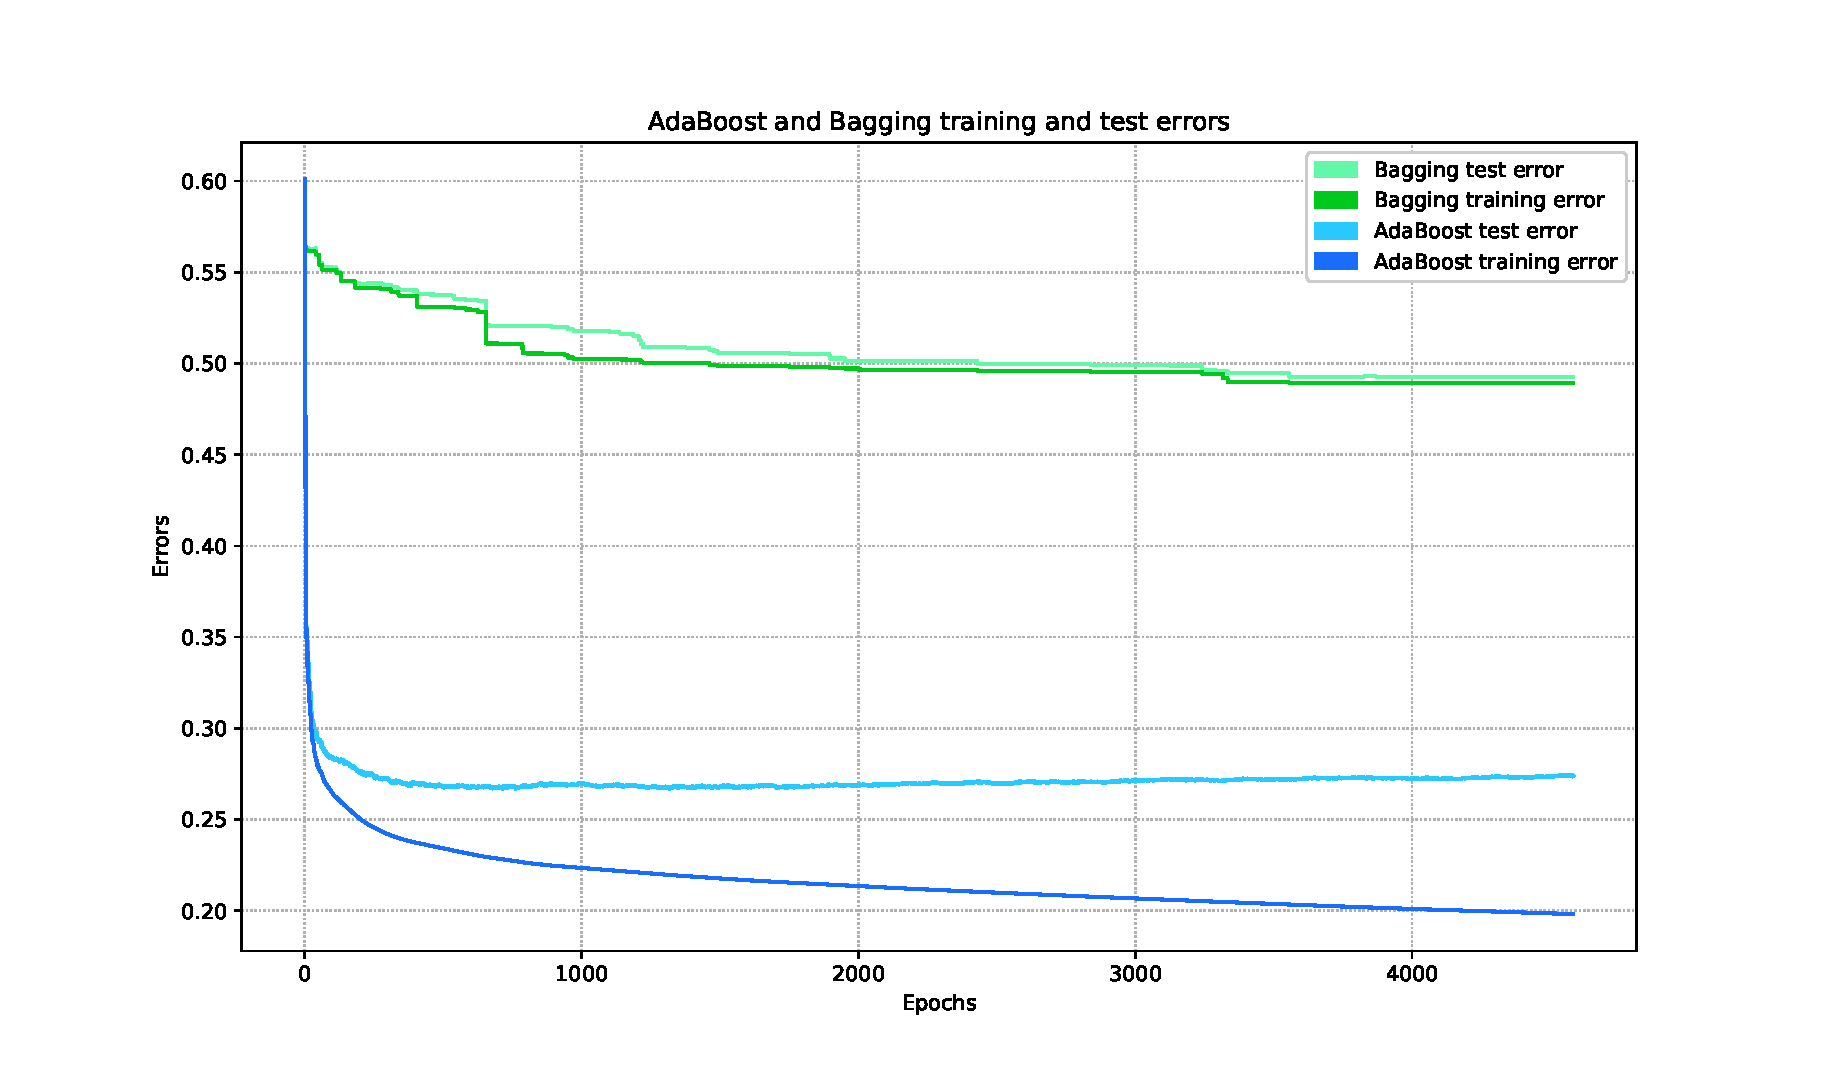
\includegraphics[width=0.5\textwidth]{figs/report_k750.eps}
	}
	\caption{\label{fig:plots_kfold}Four examples of execution over four different K-fold cross validation.}
\end{figure}
In \autoref{fig:plots_kfold}, we provide four plots of the various losses for both AdaBoost and Bagging, reporting both the training and test error over thousands of epochs with different $K$ parameters. Notice that in each of the four example provided, the AdaBoost's results suggests that the algorithm starts to overfit way before $1000$ epochs executed. On the other hand, we couldn't be able to provide the best T value for bagging algorithm with that amount of epochs.
Table \autoref{tab:results} summarize all the results for all the $K$-fold experiments on AdaBoost.

\begin{table}
\centering
\begin{tabular}{|c|c|c|}
	\hline
	K & Best T value & Test Error \\
	\hline
	2 & 144 & 0.32519 \\
	\hline
	3 & 260 & 0.30806 \\
	\hline
	5 & 873 & 0.29814 \\
	\hline
	10 & 673 & 0.30205 \\
	\hline
	20 & 650 & 0.29861 \\
	\hline
	50 & 998 & 0.29199 \\
	\hline
	150 & 637 & 0.28132 \\
	\hline
	300 & 563 & 0.27264 \\
	\hline
	750 & 714 & 0.26634 \\
	\hline
\end{tabular}
\caption{All the results varying the parameter $K$ in the cross-validation}
\label{tab:results}
\end{table}
